\documentclass[oneside,openright,uplatex]{jsbook} % oneside: 章ごとに改ページ.twoside: 章の初めが右側となるように改ページ.

% jsbookで余白が広すぎるのを直す
% 参照 https://oku.edu.mie-u.ac.jp/~okumura/jsclasses/
\setlength{\textwidth}{\fullwidth}
\setlength{\evensidemargin}{\oddsidemargin}

% OTF フォントを使えるようにし、複数のウェイトも使用可能にする。
% これがないと、Mac のヒラギノ環境で使われる角ゴが太すぎてみっともない。
\usepackage[deluxe]{otf}

% OT1→T1に変更し、ウムラウトなどを PDF 出力で合成文字ではなくす
\usepackage[T1]{fontenc}

% uplatex の場合に必要な処理 
\usepackage[utf8]{inputenc} % エンコーディングが UTF8 であることを明示する。
\usepackage[prefernoncjk]{pxcjkcat} % アクセントつきラテン文字を欧文扱いにする

% Helvetica と Times を sf と rm のそれぞれで使う。
% default だとバランスが悪いので、日本語に合わせて文字の大きさを調整する。
\usepackage[scaled=1.05,helvratio=0.95]{newtxtext}

\usepackage[dvipdfmx]{graphicx} % 画像の添付に必要
\usepackage[dvipdfmx]{color}    % 画像の添付に必要

% 表でセルを複数列で結合する
\usepackage{multicol}

% 数式の機能を拡張
\usepackage{amsmath}

% citep や citet を有効にする
\usepackage{natbib} % 参考文献を bib で管理するために必要.
\usepackage{url}    % 参考文献のリンク指定オプションに必要.

%\usepackage[hypertex]{hyperref} % url 埋め込みに必要.Usage: \href{url}{text}

% (Okumura, 2009) などを (Okumura 2009) とする
\setcitestyle{aysep={}}

% subfigure 環境で、(a)、(b) などの番号を左上に表示する。宇宙系の分野ではこれが一般的なはず。
\usepackage[nooneline]{subfigure}
\subfiguretopcaptrue

% 行番号を表示する。添削時のみに使い、事務提出版ではコメントアウトする
%\usepackage{lineno}
%\linenumbers

% PDF 内で外部リンクや文書内リンクを生成したい場合に使う(好みによる)
% \usepackage[dvipdfmx]{hyperref}

% newcommand を使うことで、繰り返し使う長ったらしい入力を簡単にすることができる
\makeatletter
\newcommand{\ion}[2]{#1$\;${\small\rmfamily\@Roman{#2}}\relax}%
\makeatother
\newcommand{\HI}{\mbox{\ion{H}{1}}} % 中性原子ガス(HI 領域)の例
\newcommand{\bs}{\symbol{92}} % backslash


%%%%%%%%%%%%%%%%%%%%%%%%%%%%%%%%%%%%%%%%%%%%%%%%%%%%%%%%%%%%%%%%%%%%%%%%%%%%%%%%%%%%%%%%%%%%%%%%%%%%%%%%%%%%%%%%%%%%%%%%%%%%%%

% 図を通し番号にする: http://rexpit.blog29.fc2.com/blog-entry-99.html
\usepackage{remreset}	% removefromreset に使う
\makeatletter
	\@removefromreset{figure}{chapter}
	\def\thefigure{\arabic{figure}}

	\@removefromreset{table}{chapter}
	\def\thetable{\arabic{table}}

	\@removefromreset{equation}{chapter}
	\def\theequation{\arabic{equation}}
\makeatother

\usepackage{comment} % \begin{comment} \end{comment}
\usepackage{color}   % {\bf \color{red}メモ}

\usepackage{natbib} % citep や citet を有効にする
\bibpunct[:]{[}{]}{,}{a}{}{,} % 括弧を () -> [] へ変更
%\usepackage[numbers]{natbib} % citep や citet を有効にする
%\bibpunct[:]{(}{)}{,}{a}{}{,}

\usepackage[]{multicol}         % 段組み % \begin{multicols}{2}%2段組み開始 ~ \end{multicols}%2段組み終了

\usepackage{wrapfig}            % 図の回り込みを許す.\begin{figure}~\end{figure} -> \begin{wrapfigure}{r}{90mm}~\end{wrapfigure} へ置き換え
                                % 直後の文が制御記号だと,回り込みに失敗し,文字が図下に重なるので,制御記号の直前に ''\noindent \ \ '' を挿入して回避する.

\renewcommand\thefootnote{\arabic{footnote})} % footnote % 脚注の調整
\usepackage{dblfnote} % 脚注を 2 段組にする

%%%%%%%%%%%%%%%%%%%%%%%%%%%%%%%%%%%%%%%%%%%%%%%%%%%%%%%%%%%%%%%%%%%%%%%%%%%%%%%%%%%%%%%%%%%%%%%%%%%%%%%%%%%%%%%%%%%%%%%%%%%%%%

\begin{document}

\begin{titlepage}


\vspace*{120truept}
\begin{center}
  \huge{学 \ 士 \ 論 \ 文 / \ 修 \ 士 \ 論 \ 文}\\
  \vspace{30truept}
%\textbf{
  \huge{タイトルが\\長い場合はいい感じに改行}\\ % title
%  \LARGE{------サブタイトル------}\\ % サブタイトル(なければコメントアウト)
%}
\vspace{100truept}
\LARGE{xx大学大学院xxxx研究科}\\
\LARGE{xxxx専攻xxxx分野xx研究室}\\
\LARGE{苗字 名前}\\
\end{center}


\end{titlepage}
 % 表紙
\thispagestyle{empty} % ページ番号を表示しない.

% レイアウトを他の章のはじめのページと揃える.
 \\
\\
\\
\\
\noindent{\Huge \sf 要旨}\\
\\
\\
\\

ハッシュテーブルは,
ハッシュ化された入力 key を配列サイズで除算した際の余り (modulo) を配列のインデックスとして値を格納することで,
key に対応する値を,定数時間で高速に取得するアルゴリズムである\footnote{コンピュータがアドレスから要素を定数時間で参照できる特性を利用している.}.
ハッシュテーブルは, key と対応した値を保持する表であることから,配列のことをテーブルと表現する.
また, key と値の対応を key-value ペアと表現する.

一般に,
ハッシュ値の剰余は配列全体に均一に分布することが望ましいが,
実際には配列の利用率を示す load factor \footnote{別名:座席利用率.} の増加に伴い衝突する.
%衝突確率を下げるには,より広い値空間に移せばよく,この操作をリハッシュと呼ぶ
%\footnote{リハッシュを行う際は,リハッシュ時間を定数時間に収めるため,通常は倍サイズの配列長に遷移させる.
%ただし,ここでの定数時間とは,繰り返し遷移させた場合のコストを1要素ごとで分割したコストが,単に O(n) となることを意味する.}
%.一般に,Chain 法.
剰余の衝突は,key-value ペアをより広い配列へ移すことで解決できる.
この操作をリハッシュと呼ぶ.
しかし,メモリ効率上,実用的な load factor を達成するためには,
リハッシュ以外の方法で衝突を解決する必要がある.

剰余衝突の解決策は,主に2種類に大別される.
1つ目は,
Chaining に代表される Open hashing\footnote{別名:Closed addressing.} である.
衝突が発生した際,新しくメモリ領域を確保し,片方向リスト\footnote{別名:linked list または singly linked list,} により現在の要素に追加する.
この手法は,
要素の削除と追加を繰り返す場合でも安定して動作するが,要素をポインタにより接続するため,
アドレス空間が連続とならず CPU キャッシュが効き難い欠点がある.
2つ目は,
Linear probing や Quadratic probing に代表される Closed hashing\footnote{別名:Open addressing.} である.
衝突が発生した際,それぞれの probing 規則に従い,隣接する空き要素に値を格納する.
Linear probing は,隣接する $1, 2, 3, ... k$ 番目の要素を線形探査する.
% 隣接する要素に値が格納されている場合は,高速に取り出せる.しかし,
配列が隙間なく埋まった場合は,
境界が分からず探査時間は大きく増加する.これを Primary clustering と呼ぶ.
% \footnote{Primary clustering と呼ぶ}.
% \href{https://en.wikipedia.org/wiki/Primary_clustering}{Primary clustering - wikipedia - 2019.06.22}}
% https://books.google.co.jp/books?id=HJ9gds_zhVEC&pg=PA186&redir_esc=y#v=onepage&q&f=false, ISBN 9780763725624 - Google Books
Quadratic probing は,隣接する $1^2, 2^2, 3^2, ... k^2$ 番目の要素を探査する.
飛び値を取るため,比較的 Primary clustering し難い.
いずれの probing も,空の要素が探査終了条件 \footnote{最悪計算量を保証するため,ホップ数を制限することもある.} の一つであるため,
要素を削除すると「要素が削除された」のか「要素が存在しない」のか判断できない.
このため,要素削除時は,削除フラグを付与する.
これらの手法は,
要素の削除と追加を繰り返す場合において,性能低下とそれに伴うリハッシュを必要とするが,
要素を隣接する要素に格納するため,CPU キャッシュが効き易い利点がある.

課題とする特性は次の通りである.
要素を挿入する際,
Open hashing は,必ず剰余値が探査すべき片方向リストの先頭アドレスを示すのに対して,
Closed hashing が示す剰余値のアドレスは probing すべき最初の要素の場合と,
挿入先の配列が使用中のため,隣接する未使用の配列に移動された要素の場合がある.
一方で,Closed hashing は Open hashing と比較してキャッシュミスを起こしにくい
\footnote{キャッシュの有効性は,全ての要素を探査する必要のある unsuccessful lookup において,特に顕著となる.
また,剰余の衝突の程度により変化する.}.
また,load factor の観点において,
Open hashing は,剰余がすべての配列番号に分布しない限り配列を使い切ることができないため,
load factor を上げるには,剰余の衝突による lookup 速度の低下を許容する必要がある.
これは,load factor と  lookup 速度がトレードオフの関係にあることを示す.
Closed hashing においても,load factor が上がるほど,配列の隙間がなくなり lookup 速度が低下する.
ただし,Quadratic probing においては特に,この速度低下は緩やかである.
\footnote{たとえば,Google は,Knuth が 80 \% 程度でリハッシュするのがよいとしている{\bf \color{red}(要出典)}とした上で,
速度を求めて google::dense\_hash\_map の load factor を 50 \% に制限している (dense\_hash\_map のコメントより).}

本研究では,既存のハッシュテーブルより lookup 速度の高い Closed hashing 手法を提案する.
まず,Closed hashing 特有の,対象となる key の剰余値自体は衝突していないにも関わらず,
これまでに衝突した隣接要素の格納先として,既に占有されている問題を解決する.
これには,
が必要となる.
そのため,た.

まず,Closed hashing の剰余値が示すアドレスに,
本来格納すべきでない隣接要素の値が格納されている場合,
必ず探査すべき要素であるように要素を入れ替える.



要素の交換には,が必要
するため,

を避けるため,Closed hashing による.

本研究では,キャッシュミスを避けるため,Closed hashing による.








\frontmatter     % make page number roman
\tableofcontents % 目次
%\listoffigures  % 図目次
%\listoftables   % 表目次

\mainmatter      % make page number arabic
\chapter{序論}
\label{chap_Introduction}

ハッシュテーブルの挙動を理解する上で,
数理モデルの示す理論的な計算量は大きな助けとなる.
図\ref{fig_taocp_v3_fig44}に\citep{knuth1998}よる比較を示す.
L は Linear probing,
U は Quadratic probing \footnote{$M \rightarrow \infty$ において,Quadratic probing と Double hashing は Uniform hashing と等価.},
S は Separate chaining の結果を示す.
図\ref{fig_taocp_v3_fig44}から分かるように,
Load factor が高くなるに従い,
平均 probe 数は上昇する傾向が見られ,
特に Linear probing では顕著である.
Quadratic probing では,
幾らか改善されるが,
いずれも
Unsuccessful lookup においては $\alpha = 0.65$ 前後,
Successful lookup においても $\alpha = 0.85$ 前後において,
急激に平均 probe 数が増加する.
この特性は,ハッシュテーブルの Load factor が閾値を超えると,
著しく性能が悪化することを意味する.
したがって,性能が悪化する手前で Load factor を制限する必要がある.
一方で,chaining を利用する C, S, SO については,
性能悪化は限られることが分かる.
このとき,
C は Coalesced Chaining\footnote{Closed hashing の一種で singly linked list により,次に辿る要素を示す.},
S は Separate chaining,
SO は Separate chaining with ordered lists である.

% Coalesced Chaining
% https://www.youtube.com/watch?v=9SPhD49ePXg
% -> singly linked list (Robin Hood の逆向きの chain.)

% taocp-v3 page.679
% As remarked above, extensive tests show that Algorithm D with two independent
% hash functions behaves essentially like uniform probing, for all practical
% purposes. In fact, double hashing is asymptotically equivalent to uniformprobing, in the limit as M → ∞ (see exercise 70).

% NOTE:   Quadratic Probing and Double Hashing have identical performance.
% Ref: 
%   page. 11
%   DatStr_152_HashTables.pdf - https://www.eecs.yorku.ca/course_archive/2003-04/F/2011/2011A/DatStr_152_HashTables.pdf

\begin{figure} % 特に強い理由がない限り、[htbp]のような指定はしないでください。
  \centering
  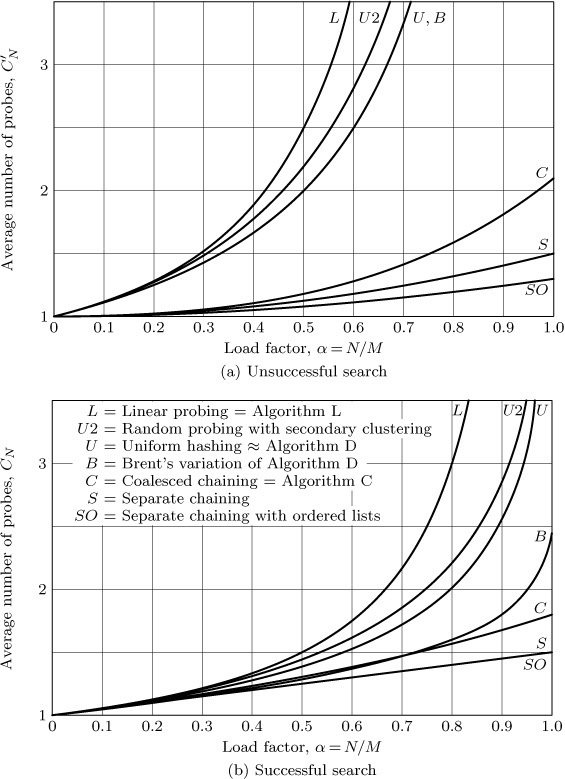
\includegraphics[width=10cm]{./figs/taocp_v3_fig44.png}
  \caption{
    Comparison of collision resolution methods: limiting values of the average number of probes as $M \rightarrow \infty$ \citep{knuth1998}.
    N は要素数,M はテーブルサイズを表す.
  }
  \label{fig_taocp_v3_fig44}
\end{figure}

%先行研究\footnote{脚注はこのように挿入します.}.

\section{先行研究}
現実的なハッシュテーブルを検討するには,
単にアルゴリズムのみならず,
対応する実実装との比較が望ましい.
ここでは,
実際に利用されているハッシュテーブルの実実装を示す.
\leavevmode \newline

{\bf std::unorderd\_map}
\samepage \\ \indent
C++ 標準のハッシュテーブル.
メモリ効率を重視しており速度は遅い.
Load factor は,しばしば 100 \% を超過する.

{\bf google::dense\_hash\_map}
\samepage \\ \indent
探査が最も高速な実装の内の 1 つで,\cite{sparsehash2005}に含まれる.
スループットで 250 query/$\mu$s 程度
\footnote{AMD Ryzen7 1700 (8C/16T) 3.7 GHz の場合.詳細は,第\ref{chap_Results}章を参照.}
の探査速度を持つことから,
探査 1 回の実行時間は 4 ns
\footnote{
  $
    250{\rm [query \slash \mu s]}
    = \frac{1}{250} {\rm [\mu s \slash query]}
    = \frac{10^3}{250} {\rm [ns \slash query]}
    = 4 {\rm [ns \slash query]}
  $
}
である.このとき,3.7 GHz の CPU では単位 clock あたりの実行時間が,
$2.7 \times 10^{-1}$ [ns/clock]
\footnote{
  $
    \frac{1}{3.7 {\rm [GHz]}}
    = \frac{1}{3.7 \times 10^9}{\rm [sec]}
    = 2.7 \times 10^{-10}{\rm [sec]}
    = 2.7 \times 10^{-1}{\rm [ns/clock]}
  $
}
であるから,1 回の探査で消費する CPU cycle は
15 clock 程度
\footnote{
  $
    \frac{ 4 {\rm [ns/query]} }{ 2.7 \times 10^{-1} {\rm [ns/clock]} }
    = \frac{ 4 }{ 2.7 \times 10^{-1} } {\rm [clock/query]}
    \simeq 15 {\rm [clock/query]}
  $
}
である.

いくつかのハッシュテーブルでは,
key のハッシュ値をテーブルサイズに丸めるために剰余演算を用いる.
整数除算に必要な CPU cycle は 14--46 clocks 程度
\footnote{
  \cite{AgnerFog2018}より AMD Ryzen7 1700 の場合.
}
であるから,dense\_hash\_map の実行時間に対して計算量が大きい.
実際に,
dense\_hash\_map では,整数除算をしておらず,
ハッシュ値の LSB \footnote{Least Significant Bit の略記.最下位ビットのこと.} から
テーブルサイズ分の bit 数だけ bit mask 演算により取り出している.
これを実現するため,テーブルサイズは常に 2 のべき乗となるように制御されている.

また,メモリ使用量を削減するため,空マークを登録する必要があり,key として使用できない.
削除マークについても同様で,key とメモリを共有しているため,削除が必要な場合は,削除マークを登録する必要があり,key として使用できなくなる.

{\bf ska::flat\_hash\_map}
\samepage \\ \indent
Robin Hood hashing の実実装の内の一つ.
条件次第で dense\_hash\_map より探査が高速であることを謳う.
Robin Hood hashing は衝突解決法の一つで,
singly linked list により,ハッシュ値の示すテーブルアドレスを示す.
本来の挿入位置が分かるため,
より近い位置に要素が移動するように調整できる.
Coalesced Chaining とは singly linked list の使い方が逆である.
実際の探査時は,Linear probing により要素を検索する.
Linear probing のコストに配慮し,
探査を $log_2(n)$ に制限している (ただし $n$ はテーブルサイズ) \cite{Skarupke2017}.

これらの特徴をまとめると,表\ref{table_hashT_cmp}のようになる.

\begin{table}[hbtp]
  \begin{center}
    \fontsize{9pt}{10pt}\selectfont
    \caption{各実装の比較.}
    \begin{tabular}{ccccccc} \hline
      \begin{tabular}{c}Implementation of\\hash table\end{tabular} & Algorism & Insert & \begin{tabular}{c}Successful\\lookup\end{tabular} & \begin{tabular}{c}Unsuccessful\\lookup\end{tabular} & Erase & \begin{tabular}{c}Memory\\efficiency\end{tabular} \rule[0pt]{0pt}{15pt} \\ \hline
      std::unorderd\_map           & Open hashing $^{a)}$   & bad   & bad  & bad  & bad   & good   \\ 
      google::dense\_hash\_map     & Closed hashing $^{b)}$ & good  & good & good & good  & medium \\
      ska::flat\_hash\_map         & Closed hashing $^{c)}$ & good  & good & good & good  & bad    \\ \hline
    \end{tabular}
    \\ 
    $^{a)}$ Chaining, 
    $^{b)}$ Quadratic probing,
    $^{c)}$ Robin Hood hashing (One of the linear probing)
    \label{table_hashT_cmp}
  \end{center}
\end{table}


\section{研究目的}

ハッシュテーブルにおいて,
単に高い探査性能を求めるだけであれば,
図\ref{fig_taocp_v3_fig44}が示すように Load factor を下げてしまえば,
どの手法も同じような性能に落ち着く.
実際に,この味付けが異なるため,
ハッシュテーブルの性能を比較する際には,
どのハッシュテーブルがどれだけのメモリを消費しているかを考慮しなくてはならず,
厳密にな比較は困難である.

しかし,現実の問題を考えるとき,
メモリ資源は有限であり,
また,高いメモリ効率を達成すれば,それだけキャッシュに乗り易くなる.
加えて,高い Load factor を達成することは,
Rehashing の発生し難い設計であることを意味し,
実利用時の安全マージンが広いことを示す.


















\chapter{Device}
\label{chap_Device}

実験装置/観測装置について説明する.タイトルは実験/観測装置の名称などにする.



\chapter{Method}
\label{chap_Method}

実験手法/解析手法/等について説明する.



\chapter{Implementation}
\label{chap_Implementation}

Implementation/実装について説明する.



\chapter{Results/Benchmarks/結果}
\label{chap_Results}

Results/Benchmarksについて記述する.



\chapter{考察}
\label{chap_Discussion}

考察について記述する.



\chapter{結論}
\label{chap_Conclusion}

結論について記述する.



\chapter*{Appendix/付録} % 章番号を出さない
\addcontentsline{toc}{chapter}{Appendix/付録} % 目次に載せる

Appendix/付録.

% 付録は chapter の 1 つとして作りますが、章番号は表示しません。
% また付録の 1 つずつはアルファベットで番号付けをするのが一般的です。
\setcounter{section}{0} % section の番号をゼロにリセットする
\renewcommand{\thesection}{\Alph{section}} % 数字ではなくアルファベットで数える
\setcounter{equation}{0} % 式番号を A.1 のようにする
\renewcommand{\theequation}{\Alph{section}.\arabic{equation}}
\setcounter{figure}{0} % 図番号
\renewcommand{\thefigure}{\Alph{section}.\arabic{figure}}
\setcounter{table}{0} % 表番号
\renewcommand{\thetable}{\Alph{section}.\arabic{table}}

\section{セクション1}
内容.

\section{セクション2}
図/表など.

\chapter*{Acknowledgments/謝辞}%
\addcontentsline{toc}{chapter}{Acknowledgments/謝辞}

感謝の気持ちを述べる.




\renewcommand{\bibname}{参考文献} % jecon.bst だと bib の doi を読み込めずエラーを吐くので,ここだけ,削除すること.
\bibliographystyle{jecon}
\nocite{*} % 文献の引用がない場合のエラーを抑制.
\bibliography{10_References}

\end{document}
